% Options for packages loaded elsewhere
\PassOptionsToPackage{unicode}{hyperref}
\PassOptionsToPackage{hyphens}{url}
%
\documentclass[
  a4paper, man, floatsintext]{apa6}
\usepackage{lmodern}
\usepackage{amssymb,amsmath}
\usepackage{ifxetex,ifluatex}
\ifnum 0\ifxetex 1\fi\ifluatex 1\fi=0 % if pdftex
  \usepackage[T1]{fontenc}
  \usepackage[utf8]{inputenc}
  \usepackage{textcomp} % provide euro and other symbols
\else % if luatex or xetex
  \usepackage{unicode-math}
  \defaultfontfeatures{Scale=MatchLowercase}
  \defaultfontfeatures[\rmfamily]{Ligatures=TeX,Scale=1}
\fi
% Use upquote if available, for straight quotes in verbatim environments
\IfFileExists{upquote.sty}{\usepackage{upquote}}{}
\IfFileExists{microtype.sty}{% use microtype if available
  \usepackage[]{microtype}
  \UseMicrotypeSet[protrusion]{basicmath} % disable protrusion for tt fonts
}{}
\makeatletter
\@ifundefined{KOMAClassName}{% if non-KOMA class
  \IfFileExists{parskip.sty}{%
    \usepackage{parskip}
  }{% else
    \setlength{\parindent}{0pt}
    \setlength{\parskip}{6pt plus 2pt minus 1pt}}
}{% if KOMA class
  \KOMAoptions{parskip=half}}
\makeatother
\usepackage{xcolor}
\IfFileExists{xurl.sty}{\usepackage{xurl}}{} % add URL line breaks if available
\IfFileExists{bookmark.sty}{\usepackage{bookmark}}{\usepackage{hyperref}}
\hypersetup{
  pdfauthor={Jana B. Jarecki},
  hidelinks,
  pdfcreator={LaTeX via pandoc}}
\urlstyle{same} % disable monospaced font for URLs
\usepackage{graphicx}
\makeatletter
\def\maxwidth{\ifdim\Gin@nat@width>\linewidth\linewidth\else\Gin@nat@width\fi}
\def\maxheight{\ifdim\Gin@nat@height>\textheight\textheight\else\Gin@nat@height\fi}
\makeatother
% Scale images if necessary, so that they will not overflow the page
% margins by default, and it is still possible to overwrite the defaults
% using explicit options in \includegraphics[width, height, ...]{}
\setkeys{Gin}{width=\maxwidth,height=\maxheight,keepaspectratio}
% Set default figure placement to htbp
\makeatletter
\def\fps@figure{htbp}
\makeatother
\setlength{\emergencystretch}{3em} % prevent overfull lines
\providecommand{\tightlist}{%
  \setlength{\itemsep}{0pt}\setlength{\parskip}{0pt}}
\setcounter{secnumdepth}{-\maxdimen} % remove section numbering
\usepackage{natbib} \usepackage{threeparttable} \usepackage{booktabs} \shorttitle{test} \usepackage{setspace} \AtBeginEnvironment{tabular}{\singlespacing} \usepackage{times} \usepackage{changes} \definechangesauthor[name={}, color=black]{jj} \definechangesauthor[name={JJ}, color=blue]{jj2} \usepackage{upgreek} \AtBeginDocument{\let\maketitle\relax}

\author{Jana B. Jarecki}
\date{11 Mai, 2020}

\begin{document}

\subsubsection{Valuation of gambles across sample sizes}

The average valuations of the gambles given the sample sizes in Study 2
resemble those in Study 1 (Table \ref{tab:means_study2}). Larger sample
sizes did not lead to systematic changes in evaluations of gambles; an
ANOVA with the predictors gamble type and gamble expected value
(\(M_0\)) outperformed one with the added predictor sample size
(\(BF_{01} = 378\)) and a sample size x gamble type interaction
(\(BF_{02} > 1000\); models with by-participant random effects).
\added[id=jj]{Unlike in Study 1 there was no substantial difference between the evaluation of \$-bet gambles  ($M=4.62, SD=3.01$) and p-bet gambles ($M=5.17, SD=4.87$); the data equally supported a model including gamble type as predictor ($M_0$) and one without gamble type as predictor, $BF_{01} = 1.54$ (both models include by-participant and by-expected-value random effects and use the valuations as the dependent variable).}

\added[id=jj]{\textit{Description versus experience.}}The valuations
from description differed from the valuations from experience for most
of the gambles and sample sizes (Table \ref{tab:means_study2}, rightmost
column). However, the finding is, especially for p-bets, less pronounced
than in Study 1. Unlike in Study 1, the \$-bets were evaluated similar
from experience (\(M=4.69, SD=3.10\)) and description
(\(M=4.83, SD=4.61\)), and the p-bets were evaluated similarly from
experience (\(M=5.25, SD=4.94\)) and description (\(M=4.32, SD=2.58\)),
the data did neither support an ANOVA with gamble-type x condition
interaction (\(M_0\)) nor a main-effects model, \(BF_{01} = 0\).

\begin{table}[tbp]

\begin{center}
\begin{threeparttable}

\caption{\label{tab:means_study2}Valuations of Gambles in Study 1}

\begin{tabular}{lccccrr}
\toprule
Condition & Sample size category & Sample size & \textit{Med} & \textit{M} & D--E & D--E:$BF\textsubscript{10}$\\
\midrule
Gamble ID 1 (\$-bet) &  &  &  &  &  & \\
\ \ \ E & xs & 5 & 5.15 & 6.29 & -0.85 & 11\\
\ \ \ E & s & 10 & 5.00 & 6.39 & -0.96 & 349\\
\ \ \ E & m & 15 & 5.95 & 6.38 & -0.95 & 71\\
\ \ \ E & l & 30 & 6.00 & 6.53 & -1.09 & 180\\
\ \ \ D & -- & -- & 4.00 & 5.43 & -- & --\\
Gamble ID 2 (\$-bet) &  &  &  &  &  & \\
\ \ \ E & xs & 6 & 4.00 & 4.55 & -0.24 & 0\\
\ \ \ E & s & 12 & 4.00 & 4.72 & -0.41 & 1\\
\ \ \ E & m & 18 & 5.00 & 4.88 & -0.57 & 4\\
\ \ \ E & l & 36 & 4.95 & 4.78 & -0.47 & 3\\
\ \ \ D & -- & -- & 3.35 & 4.31 & -- & --\\
Gamble ID 3 (\$-bet) &  &  &  &  &  & \\
\ \ \ E & xs & 7 & 8.95 & 10.65 & -1.41 & 6\\
\ \ \ E & s & 14 & 10.00 & 10.26 & -1.01 & 1\\
\ \ \ E & m & 21 & 9.70 & 10.37 & -1.12 & 2\\
\ \ \ E & l & 42 & 10.00 & 11.18 & -1.93 & 213\\
\ \ \ D & -- & -- & 6.00 & 9.25 & -- & --\\
Gamble ID 4 (p-bet) &  &  &  &  &  & \\
\ \ \ E & xs & 5 & 3.30 & 2.91 & 0.29 & 13\\
\ \ \ E & s & 10 & 3.20 & 2.94 & 0.26 & 26\\
\ \ \ E & m & 15 & 3.20 & 3.02 & 0.19 & 2\\
\ \ \ E & l & 30 & 3.20 & 3.09 & 0.11 & 0\\
\ \ \ D & -- & -- & 3.50 & 3.20 & -- & --\\
Gamble ID 5 (p-bet) &  &  &  &  &  & \\
\ \ \ E & xs & 6 & 2.00 & 1.82 & 0.10 & 1\\
\ \ \ E & s & 12 & 2.00 & 1.85 & 0.07 & 0\\
\ \ \ E & m & 18 & 2.00 & 1.85 & 0.06 & 0\\
\ \ \ E & l & 36 & 2.10 & 1.95 & -0.03 & 0\\
\ \ \ D & -- & -- & 2.00 & 1.92 & -- & --\\
Gamble ID 6 (p-bet) &  &  &  &  &  & \\
\ \ \ E & xs & 7 & 4.00 & 3.68 & 0.16 & 1\\
\ \ \ E & s & 14 & 4.10 & 3.78 & 0.07 & 0\\
\ \ \ E & m & 21 & 4.15 & 3.85 & -0.01 & 0\\
\ \ \ E & l & 42 & 4.20 & 3.90 & -0.05 & 0\\
\ \ \ D & -- & -- & 4.10 & 3.84 & -- & --\\
\bottomrule
\addlinespace
\end{tabular}

\begin{tablenotes}[para]
\normalsize{\textit{Note.} \textit{M} = mean, \textit{Med} = median, D--E = difference between mean description-based valuations and experience-based valuations, $BF\textsubscript{10}$ = Bayes Factor quantifying the evidence for a linear model $\mathrm{M}\textsubscript{1}$ predicting that valuations differ between description and experience over a linear model $\mathrm{M}\textsubscript{0}$ predicting no such differences; both models models contain a by-participant random effect. Gambles IDs 1, 2, and 3 are \$-bets; Gamble IDs 4, 5, and 6 are p-bets.}
\end{tablenotes}

\end{threeparttable}
\end{center}

\end{table}

\subsubsection{Cognitive modeling}

To gain a better insight into how sample size affects the evaluations of
the gambles we estimated the cognitive models following the same
procedure as in Study 1.

\textit{Quantitative Model Fit.} The Bayesian value updating model
described slightly more than half of the participants best (23 of 40;
57\%). The relative frequency model described 17 participants best
(42\%). The evidence strength of the models is shown in Figure
\ref{fig:fig4}. The models' mean Bayesian information criterion across
all participants equaled BIC\textsubscript{BVU}\(= -79\),
BIC\textsubscript{RF}\(= -83\), and BIC\textsubscript{BASE}\(= 49\)
(lower values indicate better fit).
\added[id = jj2]{The main  results remain unchanged when fixing the learning rate parameter in the Bayesian model to $\delta = 1$}\footnote{\added[id=jj2]{The Bayesian value updating model with $\delta=1$ described 16 of 40 (40\%) participants best; the relative frequency model described 24 participants best (60\%); the baseline model described NA participants best.}}

\begin{figure}[htb]

{\centering 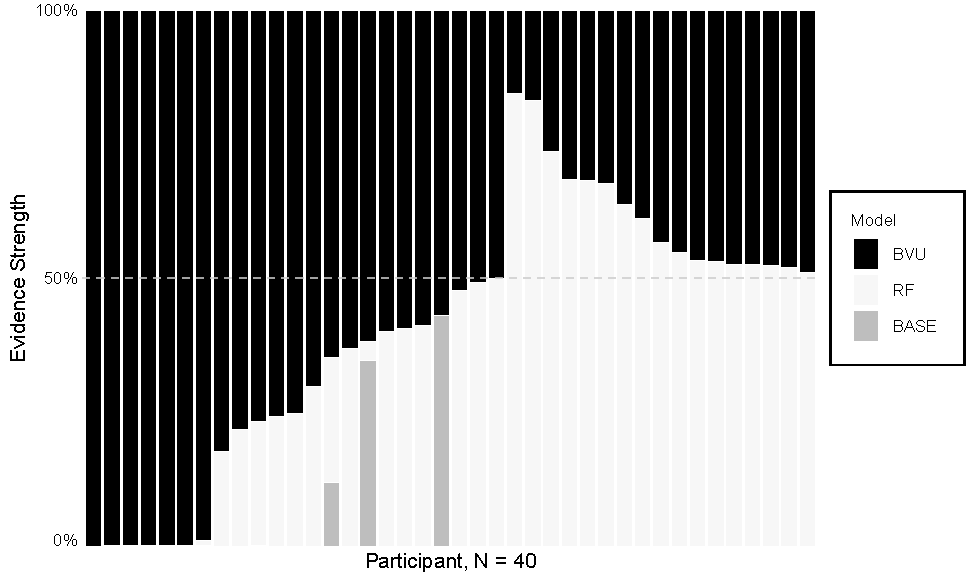
\includegraphics[width=.9\linewidth]{../figures/fig4-1} 

}

\caption{Study 2: Evidence for the models for individual participants. Darker color indicate overlapping points. \textit{RF}$=$ relative frequency model, \textit{BVU}$=$ Bayesian value updating model, \textit{BASE}$=$ Baseline model.}\label{fig:fig4}
\end{figure}

\begin{table}[tbp]

\begin{center}
\begin{threeparttable}

\caption{\label{tab:parameter_study2}Study 2: Parameter Estimates of Winning Models, \textit{M (SD)}}

\begin{tabular}{lcccc}
\toprule
Winning Model & $\tau$ & $\delta$ & $\alpha_0$ & $\sigma$\\
\midrule
BVU (\textit{n}$=$23) & 2.97 (4.55) & 2.27 (3.39) & 0.89 (0.80) & 0.23 (0.22)\\
RF (\textit{n}$=$17) & 2.15 (1.45) & -- & -- & 0.15 (0.04)\\
\bottomrule
\addlinespace
\end{tabular}

\begin{tablenotes}[para]
\normalsize{\textit{Note.} \textit{BVU}$=$ Bayesian value updating model, \textit{RF}$=$ relative frequency model. Parameters denote: $\tau=$ power utility exponent, $\alpha_0$ gain prior, $\sigma$ standard deviation.}
\end{tablenotes}

\end{threeparttable}
\end{center}

\end{table}

The estimated parameters of the models (Table
\ref{tab:parameter_study2}) reveal that, similar to Study 1, the power
utility exponent did not differ greatly between the participants that
were best described by the Bayesian value updating (BVU) model
(\(M_{\tau}= 2.97\)) and those best described by the relative frequency
model (\(M_{\alpha}=2.15\)), \(\Delta\) \(M = 0.61\) 95\% HDI
\([-1.43\), \(2.65]\), \(\mathrm{BF}_{\textrm{01}} = 2.62\). The prior
belief about the probability of a positive outcome, for participants
that were best described the BVU model, was \(B = 0.45\) (resulting from
\(\alpha = 0.89\) and \(\beta_0 = 1.11\)) and the associated learning
rate \(\delta\) was \(M_{\delta}=2.27\), indicating faster belief
updating compared to an optimal Bayesian model.

\textit{Qualitative Model Fit.} Figure \ref{fig:fig5} plots the
qualitative model fit (best-fitting model predictions against observed
evaluations by participant). As in Study 1, the data are generally
well-described by the models
(\(\added[id=jj2]{mean Pearson's} r\textsubscript{pred,obs} = 0.72\)),
except in four cases (participants s42, s54, s67, with
\(r\textsubscript{pred,obs} < 0.40\))\} where the model must be rejected
because of qualitative mis-fit.

\begin{figure}[htb]

{\centering 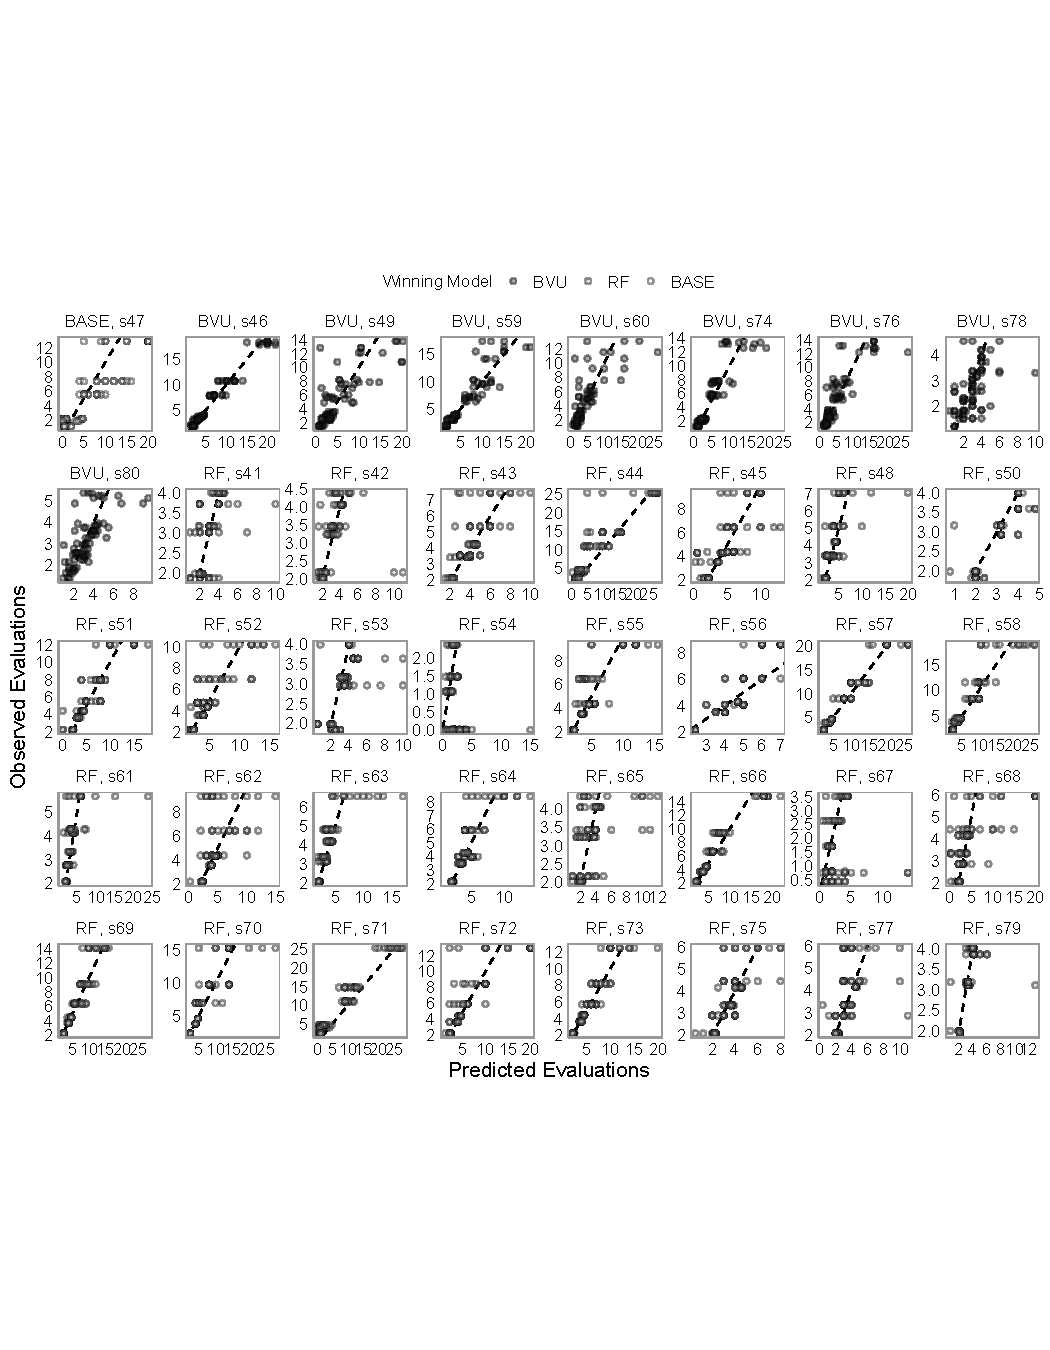
\includegraphics[width=\textwidth]{../figures/fig5-1} 

}

\caption{Study 2: Predicted evaluations from the best-fitting models plotted against the observed evaluations (by participant). Darker color indicate overlapping points. \textit{BVU}$=$ Bayesian value updating model, \textit{RF}$=$ relative frequency model.}\label{fig:fig5}
\end{figure}

\end{document}
